\chapter{Experimental Evaluation}
\label{cap:evaluation}
\section{Tele Assistance: A Self-Adaptive Service-Based System}
Tele Assistance System, also known as TAS, is a research, done by the University of York \cite{teleassist}, on self-adaptation in the domain of service-based systems. Originally introduced in \cite{valid-web-serv} has already been used in the evaluation of several self-adaptation solutions \cite{valid-web-serv}, \cite{sas-quant-ver}, \cite{dyn-qos-manage}, \cite{mod-evo-conf}, \cite{conq-compl}, albeit based on ad-hoc implementations, scenarios and evaluation metrics that make the comparison of these solutions and its use to evaluate other solution very difficult.

To address these limitation the University of York implemented TAS on their Research Service Platform (ReSeP) in conjunction with concrete scenarios in order to have an immediate use in evaluation of the self-adaptation solutions.

The system provides health support to chronic condition sufferers within the comfort of their homes. TAS uses a combination of sensors embedded in a wearable device and remote services from healthcare, pharmacy and emergency service providers. As shown in Figure \ref{fig:tas-workflow}, the TAS workflow takes periodical measurements of the vital parameters of a patient and employs a third-party medical service for their analysis. The analysis result may trigger the invocation of a pharmacy service to deliver new medication to the patient or to change his/her dose of medication, or the invocation of an alarm service leading, e.g., to an ambulance being dispatched to the patient. The same alarm service can be invoked directly by the patient, by using a panic button on the wearable device.

\begin{figure}[h]
	\centerline
	{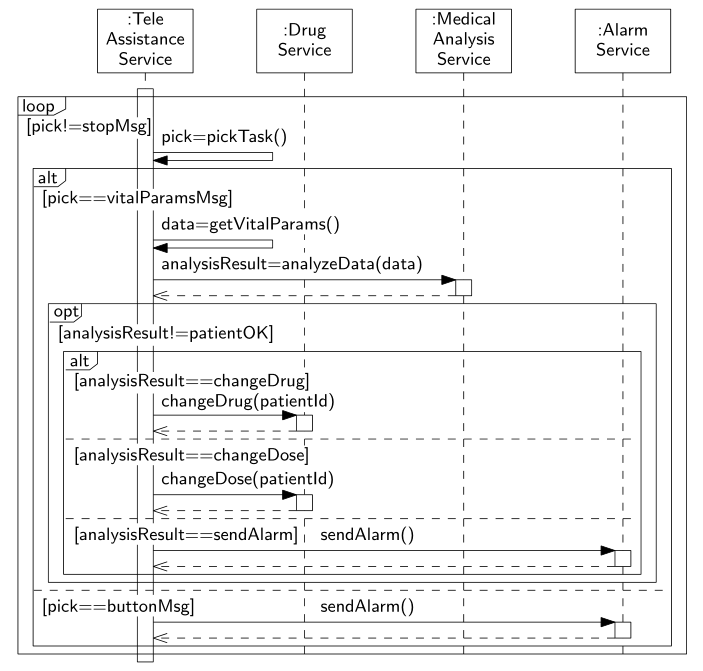
\includegraphics[scale=0.55]{img/tas-workflow.png}}
	\caption[TAS workflow]{TAS workflow}
	\label{fig:tas-workflow}
\end{figure}

They also device some generic adaptation scenarios shown in Table \ref{tab:tas-scenarios} and some metrics shown in table \ref{tab:tas-metrics}

In conclusion TAS is a reference implementation of a service based system and generic adaptation scenarios associated with different types of uncertainty. First, it aims to promote research and understanding among multiple researchers and research groups, through enabling the comparison of different self-adaptation approaches, without favouring any particular approach. Second, TAS aims to serve the advance of single research efforts by reducing the time required to evaluate self-adaptation solutions. Finally, it aims to contribute to advancing the practice of engineering self-adaptive systems, by being a realistic example of a widely used type of software system.

\begin{table}[ht!b]
	\centering
	\begin{tabular}{|l|p{3.5cm}|p{3.5cm}|p{3.5cm}|}
		\hline 
		\textbf{Scenario} & \textbf{Type of uncertainty} & \textbf{Type of adaptation} & \textbf{Type of requirements}  \\
		\hline 
		S1 & Unpredictable environment: service failure  & Switch to equivalent service; Simultaneous invocation of several services for idempotent operation & QoS: Reliability, cost \\
		\hline 
		S2 & Unpredictable environment: variation of service response time & Switch to equivalent service; Simultaneous invocation of several services for idempotent operation & QoS: Performance, cost \\
		\hline 
		S3 & Incomplete information: new service & Use new service & QoS: Reliability, performance, cost \\ 
		\hline 
		S4 & Changing requirements: new goal & Change workflow architecture; Select new service of the change on the levels & Functional: new operation \\ 
		\hline 
		S5 & Inadequate design: wrong operation sequence & Change workflow architecture & Functional: operation sequence compliance \\ 
		\hline
		
	\end{tabular} 
	\caption[TAS Scenarios]{Generic adaptation scenarios for service-based systems}
	\label{tab:tas-scenarios}
\end{table}

\begin{table}[ht!b]
	\centering
	\begin{tabular}{|p{3cm}|p{10cm}|}
		\hline 
		\textbf{Quality Attribute} & \textbf{Metrics} \\ 
		\hline 
		Reliability & Number of failed service invocations
		Number of specific operation sequence failures
		Mean time to recovery \\ 
		\hline 
		Performance & Number of specific operation sequences exceeding allowed execution time \\ 
		\hline 
		Cost & Cumulative service invocation cost over given time period \\ 
		\hline 
		Functionalities & Number of faulty process executions \\ 
		\hline 
		
	\end{tabular} 
	\caption[TAS Metrics]{Quality attributes and metrics for the evaluation and comparison of SBS self-adaptation solutions}
	\label{tab:tas-metrics}
\end{table}